\chapter{Introduction}

\section{Introduction}

Clustering is an unsupervised machine learning method that groups similar observations together. Due to its ability to find patterns in an unlabeled dataset, its an essential task in Data Mining and Knowledge Discovery. A \textit{cluster} is a group of similar instances that belongs to a \textit{centroid} (center point of a cluster). Distance-based clustering algorithms use distance measures such as Euclidean distance to calculate the similarity of datapoints. Hierarchical methods partition the instances and merge (agglomerative) or split them into bigger or smaller clusters. Many other methods exist, but this work focuses on methods for clustering \textit{mixed-type} data. \cite{mixed_type_survey_2019}

\section{k-means}

The most well known distance-based clustering method is k-means \cite{kmeans}. The goal is defined as follows: Suppose we have a finite set of $n$ instances $S=\{p_1, p_2, ..., p_n\} \in \R^m$ for a dataset with $m$ features, the target of k-means is to find optimal centroids $B=\{b_1, b_2, ..., b_k\} \subseteq \R^m$ for a given $k (\leq n) \in \N$ that minimize the sum of the squared Euclidean distance of each point in $S$ to its nearest centroid. Formally
$$\sum_{i=1}^n  d(p_i, B)$$
has to be minimized, where $d$ is the Euclidean distance from a point $p_i \in S$ to the nearest centroid in $B$ \cite{kmeans_np_hard}:
$$d(p_i, B) = min_{1 \leq j \leq k} d(p_i, b_j)$$
The Euclidean distance between two points $p$ and $q$ in an $n$-dimensional Euclidean space is defined as 
$$d(p, q) = || p - q || = \sqrt{(p_1 - q_1)^2 + (p_2 - q_2)^2 + ... + (p_n - q_n)^2}$$
Finding the optimal centroids is a NP-hard problem, even for $d=2$, as shown by Mahajan et al. \cite{kmeans_np_hard}. The most common algorithm used for the k-means problem is a iterative refinement technique proposed by Lloyd \cite{kmeans_lloyd}. It is defined as follows
\begin{enumerate} 
	\item Randomly set $k$ initial cluster centroids $b_1^{(1)}, ..., b_k^{(1)}$.
	\item Assign each obseration $p_i$ to the nearest centroid using squared Euclidean distance. This splits our instances into $S$ into $k$ sets $\{S_1^{(t)}, ..., S_k^{(t)}\}$.
	\item Recalculate the optimal position of each centroid using the mean distance to each instance assigned to the centroid: 
$$b_i^{(t+1)} = \frac{1}{|S_i^{(t)}|} \sum_{p_j \in S_i^{(t)}} p_j$$
	\item Repeat steps 2. and 3. until the centroid assignments no longer change.
\end{enumerate}

\section{Mixed-type data}

In many real-world scenarios, besides continuous, numerical data, \textit{categorial} data exists. While Euclidean distance or other distance measures work well with continuous data, categorial data is different. Suppose we have categories $\{A, B, C\}$ of a given feature, we would encode them into numeric values to allow for computation of a distance measure:
$$\{A, B, C\} \equiv \{1, 2, 3\}$$
While $A$ and $C$ can share the same semantic similarity as $A$ and $B$, numerically category $A$ and Category $C$ are now $|1-3| = 2$ apart, while Category $A$ and $B$ are only $|1-2|=1$ apart. During clustering, this could lead to instances being assigned to centroids based on a wrong distance assumption.

A possible solution is to use \textit{one-hot encoding}, also known as \textit{dummy coding} in classical statistics. One-hot encoding turns a discrete feature containing $k$ mutually exclusive categories into a vector $x$ of length $k$, in which only one of the elements $x_k$ equals 1 and all remaining elements equal 0 \cite{bishop_2006}. For an instance $B$ of a feature having $k=3$ separate categories $\{A, B, C\}$, the one-hot vector $x$ would be represented by $x = (0, 1, 0)^{\intercal}$.

\subsection{k-modes} \label{k-modes}

According to Huang \cite{kmodes}, one-hot encoding has two drawbacks:
\begin{enumerate} 
	\item In real-world applications, categorial features with hundreds or thousands of categories are encountered. This would result in a large number of binary features in the one-hot encoded representation, which will increase cost and space of computation.
	\item The centroid value of a certain one-hot encoded feature, given by a real value between 0 and 1, cannot indicate the characteristics of the according cluster, since the feature only describes the presence or absence of one category.
\end{enumerate}
Therefore, Huang \cite{kmodes} proposed using the Kronecker-Delta as a dissimilarity measure between multiple categorial columns. Formally, if we have two instances $X$ and $Y$ of a dataset with $m$ categorial features, $d_1$ will count the number of mismatches between the categorial features of both instances, defined as
$$d_1(X, Y) = \sum^m_{j=1} \delta (x_j, y_j)$$
where the Kronecker delta $\delta (x_j, y_j)$ is defined as
$$\delta (x_j, y_j) = 
\begin{cases}
    0 & (x_j = y_j)\\
    1 & (x_j \neq y_j)
\end{cases}
$$
If we have a finite set of $n$ instances $S=\{p_1, p_2, ..., p_n\}$ for a dataset with $m$ categorial features, the goal of \textit{k-modes} \cite{kmodes} is to find optimal \textit{modes} $B=\{b_1, b_2, ..., b_k\}$ for a given $k (\leq n) \in \N$ that minimize
$$\sum_{i=1}^n  d_1(p_i, B)$$
where
$$d_1(p_i, B) = min_{1 \leq l \leq k} \sum^m_{j=1} \delta (p_{i,j}, b_{l,j})$$
Similar to k-means, we can use an iterative algorithm for efficient computation \cite{kmodes}:
\begin{enumerate} 
	\item Randonly choose $k$ instances from the dataset as initial modes for the clusters.
	\item Assign each instance to their nearest mode using the proposed dissimilarity measure one by one and update the mode of each cluster after each assignment.
	\item Test if each instance still belongs to its assigned mode, i.e. if each instance is assigned to its nearest mode. If the instance would belong to a different mode, reassign the instance and update the modes of both clusters.
	\item Repeat step 3. until the mode assignments no longer change.
\end{enumerate}

\subsection{k-prototypes}

As proposed by Huang \cite{kmodes}, it is straightforward to combine the k-means and k-modes algorithms into the \textit{k-prototypes} algorithm, which can be used to cluster \textit{mixed-type} data (consisting of numerical, continuous and categorial features). The dissimilarity between two instances $X$ and $Y$ with features $A^r_1, A^r_2, ..., A^r_s, A_{s+1}^c, ..., A^c_m$, where features $A^r_1, ..., A^r_s$ are continuous and features $A_{s+1}^c, ..., A^c_m$ are categorial, is defined as
$$d_2(X,Y) = \sum^s_{j=1}(x_j - y_j)^2 + \gamma \sum^m_{j=s+1}\delta(x_j, y_j)$$
The first part of the equation is the Euclidean distance as used in k-means, while the second part is taken from the k-modes algorithm. Huang \cite{kmodes} states: "The weight $\gamma$ is used to avoid favouring either type of attribute".

Again, we need to find $k$ optimal centroids $B=\{b_1, b_2, ..., b_k\}$ and therefore have to minimize
$$\sum_{i=1}^n  d_2(p_i, B)$$
where
$$d_2(p_i, B) = min_{1 \leq l \leq k} \sum^s_{j=1}(p_{i,j} - b_{l,j})^2 + \gamma \sum^m_{j=s+1}\delta(p_{i,j}, b_{l,j})$$
We can minimize both distance measures at the same time since they are nonnegative. Therefore, we can use the same algorithm as defined in \ref{k-modes}. \cite{kmodes}

\subsection{Gower distance}

\textit{Gower Distance} \cite{gower} is a general similarity measurement between instances containing mixed-type features. It is defined as follows: When comparing instances $x_i$ and $x_j$, for each feature $k$ of $p$ total features, we calculate a score $s_{ijk} \in [0,1]$. The score will be close to 1 for two instances $x_{ik}$ and $x_{jk}$ of a feature $k$ if they are similar, and close to 0 they are not similar.
Gower distance is also computable between instances with missing values, therefore a quantity $\delta_{ijk}$ is calculated, which is equal to 1, when feature $k$ can be compared across the two instances $x_i$ and $x_j$, and 0 otherwise (illustrated in Figure \ref{gower_dichotomous}).
Gower distance then is the average of the known score
$$S_{ij} = \frac{\sum^p_{k=1}s_{ijk}\delta_{ijk}}{\sum^p_{k=1}\delta_{ijk}}$$
The Score $s_{ijk}$ is calculated differently according to the type of feature \cite{gower}:
\begin{enumerate}
	\item For \textit{dichotomous} (when a value is either present or absent) features, the score $s_{ijk}$ is 1 when the value is present in both features and 0 otherwise, as shown in Figure \ref{gower_dichotomous}.
	\item For categorial features, the score $s_{ijk}$ is 1 if they both instances match on feature $k$ and 0 otherwise.
	\item For continuous features the score is calculated as
	$$s_{ijk} = 1-\frac{|x_i-x_j|}{R_k}$$
	where $R_k$ is the range of feature $k$ in the dataset or in the sample.
\end{enumerate}
\begin{figure}
	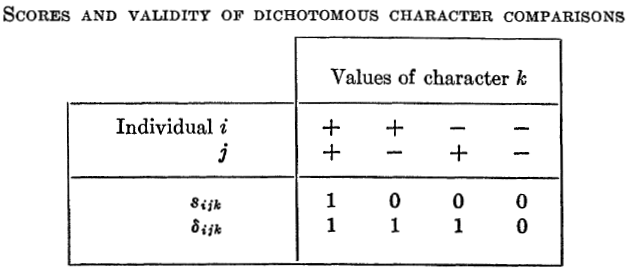
\includegraphics[width=\linewidth]{gower-dichotomous.png}
	\caption{Score $s_{ijk}$ and quantity $\delta_{ijk}$ of a feature $k$ on two instances $x_i$ and $x_j$. Presence of a feature is denoted by "+" and absence by "-". \cite{gower}}
	\label{gower_dichotomous}
\end{figure}
Gower \cite{gower} has shown that $\sqrt{1- S_{ij}}$ is a valid distance representation for two instances $x_i$ and $x_j$. We can now convert our similarity matrix $S$ into a distance matrix and are able to use Hierarchical clustering methods \cite{algorithms_for_clustering_data}. Philip and Ottaway \cite{philip_ottaway} used Gower distance with agglomerative clustering. Agglomerative clustering places each object into its own cluster and recursively merges the clusters together using the given distance matrix, until only the specified number of clusters is remaining \cite{algorithms_for_clustering_data}.


\section{Methodology}

In this work we use 8 mixed-type datasets from the UC Irvine Machine Learning Repository \cite{uci_ml_rpo}. 
The Abalone dataset \cite{abalone} contains physical measurements from abalones. It has 4177 instances, one categorial feature and seven continuous features.
The Auction Verification dataset \cite{auction_verification} has 2043 instances that contain verification runs of multi-round auctions. It is composed of six categorial and one continuous feauture.
The Bank Marketing dataset \cite{bank_marketing} is related to a direct marketing campaign of a portuguese banking institution. It has 49732 instances. The "age", "day" and "month" features were removed, which results in eight categorial and five continuous features.
The Breast Cancer dataset \cite{breast_cancer} contains 699 instances and 9 categorial features.
The Census Income dataset \cite{census_income} has a total of 48842 instances. It is composed of eight categorial and 6 continuous features.
The Credit Approval dataset \cite{credit_approval} contains information of applications for credit cards. It has 690 instances, nine categorial features and six continuous features.
The Heart Disease dataset \cite{heart_disease} is composed of four datasets and has 920 instances in total. It has seven categorial features and six continuous features.
The Soybean (Large) Dataset \cite{abalone} consists of 683 instances from soybeans with a certain disease and has 35 categorial features.

All instances containing missing values were removed. Duplicate instances were explicitly not removed, since there is no information available if they are duplicates by accident, or real duplicates. Categorial columns were standardized by removing the mean and scaling to unit variance, using the scikit-learn Python API \cite{scikit_learn}. Formally, the standardized score $z$ of a sample $x$ from a feature is calculated as
$$z = \frac{(x-\mu)}{\sigma}$$
where $\mu$ is the mean of the samples $x_1, ...,x_N$ from a feature of length $N$, defined as
$$\mu = \frac{1}{N} \sum^{N}_{i=1} x_i$$
and $\sigma$ is the standard deviation of the samples of a feature, defined as
$$\sigma = \sqrt{\frac{1}{N} \sum^{N}_{i=1}(x_i - \mu)^2}$$
The datasets were shuffled. For all random operations, a random state of integer value 0 was used to ensure reproducibility.





\section{Comparison of classical Clustering methods}

\begin{figure}
\begin{center}
\scalebox{0.8}{
\begin{tabular}{|c|c|c|c|c|}
\hline
&Naive k-means&k-means one-hot&k-prototypes&Gower distance\\\hline
Abalone&0.171795&\bf{0.173982}&0.171639&0.161416 \\ \hline
Auction Verification&\bf{0.016172}&0.007087&0.007667&0.006170 \\ \hline
Bank Marketing&0.019781&\bf{0.026060}&0.019522&0.001334 \\ \hline
Breast Cancer&\bf{0.746818}&0.736310&0.592480&0.553707 \\ \hline
Census Income&0.108029&\bf{0.184979}&0.141737&0.004259 \\ \hline
Credit Approval&\bf{0.313076}&0.171038&0.116579&0.003465 \\ \hline
Heart Disease&\bf{0.204577}&0.164486&0.189264&0.140792 \\ \hline
Soybean Disease&0.672229&\bf{0.710164}&0.567635&0.669526 \\
\hline
\end{tabular}
}
\end{center}
\caption{Comparsion of Normalized Mutual Information of various classical methods on clustering mixed-type datasets.}
\label{classical_comparison_nmi}
\end{figure}

\begin{figure}
\begin{center}
\scalebox{0.8}{
\begin{tabular}{|c|c|c|c|c|}
\hline
&Naive k-means&k-means one-hot&k-prototypes&Gower distance\\\hline
Abalone&0.135265&0.131434&0.134307&\bf{0.195356} \\ \hline
Auction Verification&0.664709&0.576114&0.580519&\bf{0.800783} \\ \hline
Bank Marketing&0.779600&0.786600&0.787200&\bf{0.884200} \\ \hline
Breast Cancer&\bf{0.960469}&0.950220&0.915081&0.900439 \\ \hline
Census Income&0.608200&0.697600&0.625600&\bf{0.768400} \\ \hline
Credit Approval&\bf{0.808576}&0.705972&0.666156&0.548239 \\ \hline
Heart Disease&0.334448&0.321070&0.424749&\bf{0.565217} \\ \hline
Soybean Disease&0.576512&\bf{0.599644}&0.471530&0.501779 \\
\hline
\end{tabular}
}
\end{center}
\caption{Comparsion of Cluster Accuracy of various classical methods on clustering mixed-type datasets.}
\label{classical_comparison_acc}
\end{figure}

\chapter{Neural Networks}

The idea of computation by neurons inspired by the human brain was first formalized into a mathematical model by McCulloch \cite{neural_network_1943}. A \textit{neuron} was defined as a element that takes multiple boolean inputs and has one boolean output. The neuron \textit{fires}, meaning the output is set to true, when the sum of the input values extends a certain threshold.

The first single-layer \textit{perceptron}, the first neural machine learning algorithm, was invented by Rosenblatt \cite{perceptron}. It is a function $f$ that maps a input vector $x \in \R$ to a single binary valued ouput, which is then used to classify the input. Formally, $f$ is defined as
$$f(x_i) = 
\begin{cases}
    1 & \sum_i w_{ij}x_i + b > 0\\
    0 & otherwise
\end{cases}
$$
where $w$ is the learnable weight matrix, and $b$ is a predefined bias. For training, the weights $w$ are simply incremented when the output is 0 but the ground truth is 1, and decremented if the output is 1 but should be 0. If the output was predicted right, no weights are changed.

\chapter{Autoencoders}
\chapter{Deep clustering methods}
\chapter{Attention}
\section{Comparison of deep clustering methods}
\chapter{Conclusion}